%===============================================================================
% LaTeX sjabloon voor de bachelorproef toegepaste informatica aan HOGENT
% Meer info op https://github.com/HoGentTIN/bachproef-latex-sjabloon
%===============================================================================

\documentclass{bachproef-tin}

\usepackage{hogent-thesis-titlepage} % Titelpagina conform aan HOGENT huisstijl
\usepackage{graphicx} 
\usepackage{tabularx}
\usepackage{lscape}
\usepackage{verbatim}
%%---------- Documenteigenschappen ---------------------------------------------
% TODO: Vul dit aan met je eigen info:

% De titel van het rapport/bachelorproef
\title{Een analyse van z/OS Health Checker en hoe deze te optimaliseren}

% Je eigen naam
\author{Jonas Braem}

% De naam van je promotor (lector van de opleiding)
\promotor{Thomas Pollet}

% De naam van je co-promotor. Als je promotor ook je opdrachtgever is en je
% dus ook inhoudelijk begeleidt (en enkel dan!), mag je dit leeg laten.
\copromotor{Kevin Somers}

% Indien je bachelorproef in opdracht van/in samenwerking met een bedrijf of
% externe organisatie geschreven is, geef je hier de naam. Zoniet laat je dit
% zoals het is.
\instelling{HCL Technologies}

% Academiejaar
\academiejaar{2019-2020}

% Examenperiode
%  - 1e semester = 1e examenperiode => 1
%  - 2e semester = 2e examenperiode => 2
%  - tweede zit  = 3e examenperiode => 3
\examenperiode{2}

%===============================================================================
% Inhoud document
%===============================================================================

\begin{document}

%---------- Taalselectie -------------------------------------------------------
% Als je je bachelorproef in het Engels schrijft, haal dan onderstaande regel
% uit commentaar. Let op: de tekst op de voorkaft blijft in het Nederlands, en
% dat is ook de bedoeling!

%\selectlanguage{english}

%---------- Titelblad ----------------------------------------------------------
\inserttitlepage

%---------- Samenvatting, voorwoord --------------------------------------------
\usechapterimagefalse
%%=============================================================================
%% Voorwoord
%%=============================================================================

\chapter*{\IfLanguageName{dutch}{Woord vooraf}{Preface}}
\label{ch:voorwoord}

%% TODO:
%% Het voorwoord is het enige deel van de bachelorproef waar je vanuit je
%% eigen standpunt (``ik-vorm'') mag schrijven. Je kan hier bv. motiveren
%% waarom jij het onderwerp wil bespreken.
%% Vergeet ook niet te bedanken wie je geholpen/gesteund/... heeft

Deze proef is geschreven in het kader van het voltooien van de richting Toegepaste Informatica met keuzetraject Mianframe-beheer en Applicaties. Dit vond ik een interessant onderwerp omdat de mainframe me intrigeert en Health Checker was ook iets dat nog niet binnen de opleiding besproken was maar dat mij wel interesseerde. Ik vond deze proef ook zeer speciaal omdat mijn proef heeft bijgedragen aan een systeem dat nu geïmplementeerd is door de opdrachtgever. Ook het feit dat ik niks kende van het onderwerp was iets wat me aansprak om zo mijn kennis van de mainframe te verrijken. Deze proef is er wel niet zomaar gekomen en daarom wil ik nog enkele mensen bedanken voor hun bijdrage aan deze Bachelorproef.

De eerste persoon die ik wil bedanken is Kevin Somers voor de hulp en ondersteuning doorheen de gehele bachelorproef. Ik kon altijd terecht bij hem met vragen. En heb van hem ook nog veel geleerd over de Mainframe. Verder stond hij ook klaar om elke week te bellen om de proef te bespreken. Ik wil ook de Zweedse collega van Kevin, Bengt Gellingskog bedanken om samen met Kevin mij te ondersteunen met deze proef tijdens onze discussies over de Health Checker setup. Verder wil ik ook nog de andere collega's waaronder Louis Huysman en Alain de Waele van HCL te zuiderpoort bedanken en HCL Technologies BVBA zelf voor de mogelijkheid om deze proef te doen binnen hun infrastructuur.

Ik wil ook mijn promotor Thomas Pollet bedanken voor zijn feedback op de inhoud van mijn bachelorproef.

Tot slot wil ik ook mijn ouders bedanken voor de steun om mijn opleiding en mijn bachelorproef te voltooien. Waaronder de feedback op de schrijfwijze van mijn proef.

Ik wens u veel plezier toe bij het lezen van deze proef.
%%=============================================================================
%% Samenvatting
%%=============================================================================

% TODO: De "abstract" of samenvatting is een kernachtige (~ 1 blz. voor een
% thesis) synthese van het document.
%
% Deze aspecten moeten zeker aan bod komen:
% - Context: waarom is dit werk belangrijk?
% - Nood: waarom moest dit onderzocht worden?
% - Taak: wat heb je precies gedaan?
% - Object: wat staat in dit document geschreven?
% - Resultaat: wat was het resultaat?
% - Conclusie: wat is/zijn de belangrijkste conclusie(s)?
% - Perspectief: blijven er nog vragen open die in de toekomst nog kunnen
%    onderzocht worden? Wat is een mogelijk vervolg voor jouw onderzoek?
%
% LET OP! Een samenvatting is GEEN voorwoord!

%%---------- Nederlandse samenvatting -----------------------------------------
%
% TODO: Als je je bachelorproef in het Engels schrijft, moet je eerst een
% Nederlandse samenvatting invoegen. Haal daarvoor onderstaande code uit
% commentaar.
% Wie zijn bachelorproef in het Nederlands schrijft, kan dit negeren, de inhoud
% wordt niet in het document ingevoegd.

\IfLanguageName{english}{%
\selectlanguage{dutch}
\chapter*{Samenvatting}
\lipsum[1-4]
\selectlanguage{english}
}{}

%%---------- Samenvatting -----------------------------------------------------
% De samenvatting in de hoofdtaal van het document

\chapter*{\IfLanguageName{dutch}{Samenvatting}{Abstract}}
De mainframe is een vitaal onderdeel van verscheidene belangrijke sectoren. Ze worden voornamelijk gebruikt door hun garantie van continue toegankelijkheid. Er is zowel software als hardware speciaal ontworpen voor dit doeleind. z/OS Health checker is een voorbeeld van software dat hiervoor gebruikt wordt. Dit is een preventie tool die problemen probeert op te sporen voordat ze gebeuren. Maar de logging hiervan is niet zo efficiënt en de standaardopstelling van deze tool is ook niet efficiënt voor elke opstelling van en mainframe. Dit is ook het geval bij de opstelling HCL Technologies BVBA het doel van deze proef is die opstelling optimaliseren en een veel efficiëntere manier van logging opstellen. Er wordt eerst gekeken naar structuur binnen de mainframe waar z/OS health checker opereert. Dan naar de opstelling van z/OS Health Checker zelf en een analyse van die opstelling binnen HCL Technologies BVBA. Dan zal er een efficiëntere logging opgezet worden via JCL - jobs met als vervolg een optie deze om te zetten naar een Web interface.


%---------- Inhoudstafel -------------------------------------------------------
\pagestyle{empty} % Geen hoofding
\tableofcontents  % Voeg de inhoudstafel toe
\cleardoublepage  % Zorg dat volgende hoofstuk op een oneven pagina begint
\pagestyle{fancy} % Zet hoofding opnieuw aan

%---------- Lijst figuren, afkortingen, ... ------------------------------------

% Indien gewenst kan je hier een lijst van figuren/tabellen opgeven. Geef in
% dat geval je figuren/tabellen altijd een korte beschrijving:
%
%  \caption[korte beschrijving]{uitgebreide beschrijving}
%
% De korte beschrijving wordt gebruikt voor deze lijst, de uitgebreide staat bij
% de figuur of tabel zelf.

\listoffigures
\listoftables

% Als je een lijst van afkortingen of termen wil toevoegen, dan hoort die
% hier thuis. Gebruik bijvoorbeeld de ``glossaries'' package.
% https://www.overleaf.com/learn/latex/Glossaries

%---------- Kern ---------------------------------------------------------------

% De eerste hoofdstukken van een bachelorproef zijn meestal een inleiding op
% het onderwerp, literatuurstudie en verantwoording methodologie.
% Aarzel niet om een meer beschrijvende titel aan deze hoofstukken te geven of
% om bijvoorbeeld de inleiding en/of stand van zaken over meerdere hoofdstukken
% te verspreiden!

%%=============================================================================
%% Inleiding
%%=============================================================================

\chapter{\IfLanguageName{dutch}{Inleiding}{Introduction}}
\label{ch:inleiding}

Men zal het niet beseffen maar zonder de Mainframe zouden veel hedendaagse diensten wegvallen. Ook al is de mainframe voor velen iets uit het verleden, veel sectoren blijven er op vertrouwen. Een voorbeeld zijn de bankinstellingen, de kans is groot dat als je iets betaalt met je bankkaart dat de transactie verwerkt wordt door een mainframe. Een ander voorbeeld zijn de vliegmaatschappijen, als je eens een kijkje zou kunnen nemen naar de computer die gebruikt wordt op de luchthaven om je in te checken op je vlucht, zal je merken dat dit hoogstwaarschijnlijk een terminal is die aangesloten zit op een Mainframe. Verder wordt de mainframe ook nog gebruikt in andere sectoren zoals:


\begin{itemize}
  \item Financiële Sector
  \item Magazijnbeheer
  \item Verzekeringen
  \item Ziekenzorg
  \item Overheid
  \item \ldots
\end{itemize}

Een uitval van een mainframe kan dus kritische diensten laten wegvallen. Bijvoorbeeld de mogelijkheid tot overschrijven via de bank. Daarom is een van de belangrijkste factoren van de mainframe de beschikbaarheid. De mainframe garandeert een uptime van 24 op 24, 7 op 7, 365 op 365 het hele jaar door dus. Hiervoor worden verscheidene technieken gebruikt zoals de "alles 2 regel". Je zult in een mainframe alles dubbel terugvinden. Ook de architectuur binnen de mainframe, de Parallel Sysplex(Meer hierover in hoofdstuk \ref{ch:stand-van-zaken}) zorgt dat bij een uitval van 1 partitie een andere zijn workload direct overneemt.an zijn er binnen die architectuur ook nog verschillende software componenten die hier voor zorgen. Een daarvan is degene waar deze proef zich op focust z/OS Health Checker, deze tool werkt preventief. Het zal proberen om de problemen op te sporen alvorens die plaats vinden en zal de System Administrator hiervan verwittigen. In hoofdstuk \ref{ch:stand-van-zaken} zal de werking hiervan tot in detail worden uitgelegd.

\section{\IfLanguageName{dutch}{Probleemstelling}{Problem Statement}}
\label{sec:probleemstelling}

De z/OS Health Checker opstelling van HCL Technologies is al lang niet meer veranderd en is ook niet gestandaardiseerd over de verschillende partities binnen de Mainframe. Bij eventuele uitbreiding van het systeem is er dus ook niet direct een standaardopstelling die men kan toepassen. Verder vind er ook een inefficiënte logging plaats. Deze is nu niet echt aanwezig, de bedoeling is dat de verantwoordelijke van elke partitie een log krijgt van alle fouten binnen zijn partitie.

\section{\IfLanguageName{dutch}{Onderzoeksvraag}{Research question}}
\label{sec:Hoofdonderzoeksvraag}

Deze proef zal zich focussen op de z/OS Health checker opstelling van HCL technologies met volgende onderzoeksvraag.

\begin{itemize}
	\item Is het mogelijk een standaardopstelling te maken voor een z/OS Health Checker omgeving?
\end{itemize}

\subsection{Deelonderzoeksvragen}
\label{subsec:Deelonderzoeksvragen}

Daarnaast is er in deze proef ook een focus op verdere efficiëntere logging van z/OS Health Checker en of deze kan via een webUI. Daaruit volgen de deelonderzoeksvragen:

\begin{itemize}
	\item Kan er een efficiënt log-systeem opgezet worden voor de z/OS Health Checker output?
\end{itemize}


\section{\IfLanguageName{dutch}{Onderzoeksdoelstelling}{Research objective}}
\label{sec:onderzoeksdoelstelling}

Het doel van deze proef is om een standaardopstelling te bekomen van z/OS Health Checker binnen de omgeving van HCL Technologies zodat deze bij uitbreiding van het systeem deze onmiddellijk kan implementeren op nieuwe partities.

Verder is het doel om ook een duidelijke logging op te stellen voor elke verantwoordelijke van elke logische partitie van de Mainframe omgeving van HCL, met als eventueel vervolg een mogelijkheid te vinden om die logging te laten gebeuren via een web interface.

\section{\IfLanguageName{dutch}{Opzet van deze bachelorproef}{Structure of this bachelor thesis}}
\label{sec:opzet-bachelorproef}

% Het is gebruikelijk aan het einde van de inleiding een overzicht te
% geven van de opbouw van de rest van de tekst. Deze sectie bevat al een aanzet
% die je kan aanvullen/aanpassen in functie van je eigen tekst.

De rest van deze bachelorproef is als volgt opgebouwd:

In Hoofdstuk~\ref{ch:stand-van-zaken} wordt een overzicht gegeven van de stand van zaken binnen het onderzoeksdomein, op basis van een literatuurstudie.

In Hoofdstuk~\ref{ch:methodologie} wordt de methodologie toegelicht en worden de gebruikte onderzoekstechnieken besproken om een antwoord te kunnen formuleren op de hoofdonderzoeksvraag en de 1ste deelonderzoeksvraag.

In hoofdstuk~\ref{ch:Vervolg op bachelorproef} word er gekeken naar eventuele vervolgen voor deze bachelor proef.


% TODO: Vul hier aan voor je eigen hoofstukken, één of twee zinnen per hoofdstuk

In Hoofdstuk~\ref{ch:conclusie}, tenslotte, wordt de conclusie gegeven en een antwoord geformuleerd op de onderzoeksvragen. Daarbij wordt ook een aanzet gegeven voor toekomstig onderzoek binnen dit domein.
\chapter{\IfLanguageName{dutch}{Stand van zaken}{State of the art}}
\label{ch:stand-van-zaken}

% Tip: Begin elk hoofdstuk met een paragraaf inleiding die beschrijft hoe
% dit hoofdstuk past binnen het geheel van de bachelorproef. Geef in het
% bijzonder aan wat de link is met het vorige en volgende hoofdstuk.

% Pas na deze inleidende paragraaf komt de eerste sectiehoofding.

Dit onderzoek zal zich focussen op z/OS Health Checker. Dit is een tool die draait in een mainframe omgeving. Vooraleer we kunnen beginnen met het bespreken van de oplossingsmethode van de onderzoeksvragen moeten we ons eerst verdiepen in de mainframe zelf en de omgeving waarin z/OS Health Checker draait om zo duidelijk te maken waarom deze tool zijn aanwezigheid belangrijk is en hoe deze werkt. Verder moeten we ook de basis begrijpen van andere tools en systemen binnen de mainframe zoals ISPF, SDSF en JES. Om daarna te eindigen met JCL de taal die word gebruikt om de z/OS Health Checker logs op te stellen.

\section{De Mainframe}
\label{sec:De Mainframe}

De Mainframe speelt een centrale rol in de dagelijkse operaties bij de meeste grote bedrijven. De Ontwikkeling van de mainframe gaat terug tot de jaren '50. Ook al is er door de jaren heen veel veranderd aan de mainframe blijft het het meest stabiele,veilige en compatibele computing platform. Desondanks dat de mainframe een grote aanwezigheid heeft binnen de financiële wereld, blijft deze vrij onzichtbaar voor de grote menigte. Maar eigenlijk zijn we bijna allemaal indirect mainframe gebruikers ook al realiseren we het niet. (\cite{Ebbers2011})

Een mainframe is een computer die gebruikt wordt door vooral grote bedrijven voor kritieke applicaties(bijvoorbeeld geld transacties bij een bank), of voor het verwerken van grote hoeveelheid data(bijvoorbeeld de gehele voorraad van een bedrijf beheren). De mainframe is voor zulke operaties geschikt omdat het gespecialiseerd is voor het afhandelen van Input-Output transacties, een mainframe kan er tot 30000 afhandelen per seconde. En dit hoog niveau van data verwerking is zeker nodig, probeer je maar eens in te beelden hoeveel geld transacties er op 1 dag plaatsvinden. Een groot verschil van een mainframe tegenover een server is de hardware. In een mainframe kunnen er tegenwoordig 100 processors aanwezig zijn. Een ander verschil is dat de mainframe een langere uptime heeft. Het is niet speciaal dat een mainframe langer dan 10 jaar continu draait. Verder is een mainframe ook fysiek veel groter dan één enkele server(zie figuur \ref{fig:mainframe}).\cite{Ebbers2011}

\begin{figure}[h]
	\centering
	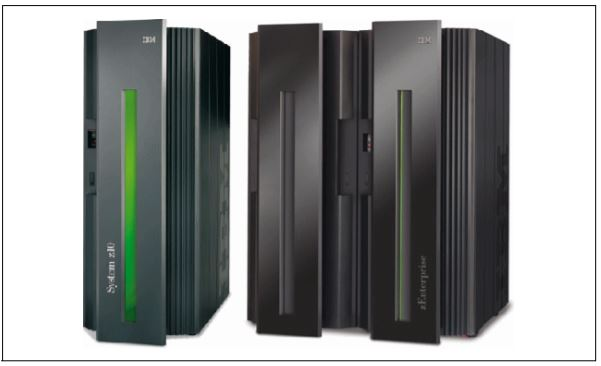
\includegraphics{img/mainframe}
	\caption[Mainframe]{{\small \textit{2 mainframes de System z Business Class en Enterprise class(\cite{Ebbers2011})}}}
	\label{fig:mainframe}
\end{figure}

Men mag bij de term mainframe wel niet denken aan een supercomputer. Het grote verschil tussen de 2 is dat een mainframe gespecialiseerd is in het afhandelen van transacties en het verwerken van data. Terwijl een supercomputer gespecialiseerd is in het maken van wiskundige berekeningen.

\section{Logische partities en de Parallel Sysplex}
\label{sec:Logische partities en de Parallel Sysplex}

Nu men weet wat een mainframe is, is het belangrijk om te kijken naar de architectuur binnen het systeem zelf. Dit is aan de hand van allerlei gekoppelde logische partities die men als geheel de Parallel Sysplex noemt. Dit is ook de omgeving waarin z/OS Health Checker opereert. Daarom belichten we ook deze componenten in dit hoofdstuk.

\subsection{Logische partitie of LPAR}
\label{subsec:Logische partitie of LPAR}
De IBM mainframe kan verdeeld worden in verscheidene logische systemen. Tussen deze systemen kan men volgende resources verdelen:
\begin{itemize}
	\item Memory
	\item Processors
	\item Input-Output devices.
\end{itemize}
Deze aparte systemen noemt men een logische partitie of LPAR. Al deze LPARs staan onder de controle van een hypervisor. De hypervisor is een software laag voor het beheer van meerdere besturingssystemen. De Verdeling van resources gebeurt door de Processor Resource/Systems Manager(PR/SM)(zie figuur \ref{fig:lpar}). De volledige definitie van een LPAR luidt als volgt: Een subset van de processor hardware dat gedefinieerd is voor het ondersteunen van een besturingssysteem. Meerdere LPARs zijn dus gelijkaardig aan verschillende aparte mainframes. Ze hebben elk hun eigen besturingssysteem en toegewezen hardware. (\cite{Ebbers2011})

\begin{figure}[h]
	\centering
	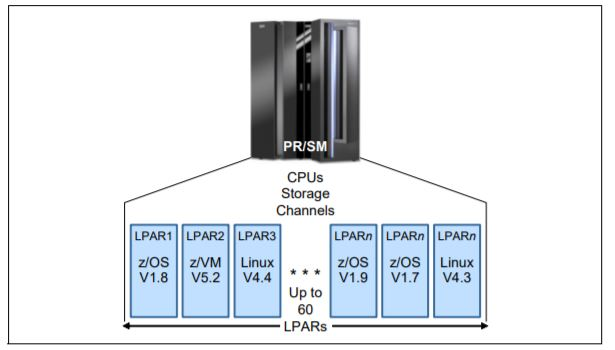
\includegraphics{img/LPAR}
	\caption[Logische Partities]{{\small \textit{Visualisatie van logische partities(\cite{Ebbers2011})}}}
	\label{fig:lpar}
\end{figure}


\subsection{Parallel Sysplex}
\label{subsec:Parallel Sysplex}

De Parallel Sysplex is een een techniek van clusteren. Waarmee men meerdere LPARs groepeert.  z/OS Health Checker zal zowel opereren op aparte LPAR als op de gehele Parallel Sysplex door globale checks(meer hierover in sectie \ref{sec:z/OS Health Checker}). Daarvoor gaan we ons ook verdiepen in deze clustering techniek.

Sysplex staat voor SYStems comPLEX dit is een of meerdere LPARs met z/OS, samengevoegd als 1 unit die gespecialiseerde hardware en software gebruikt. Het gebruikt unieke messaging services en kan bestandsstructuren delen in de couple facilty(CF) datasets. Een sysplex is een instantie van een computer systeem dat draait op 1 of meerdere fysieke partities waarvan elke een andere release kan draaien van het z/OS besturingssysteem. Een sysplex is wel geïsoleerd tot 1 fysieke mainframe. De Parallel Sysplex anderzijds laat meerdere mainframes zich voordoen als 1 systeem. (\cite{Ebbers2011}) 

Een Parallel Sysplex is een symmetrische sysplex die gebruik maakt van het delen van data met meerdere systemen. Dit is dus de clustering van meerder mainframes. We bespreken ook enkele protocollen die de Parallel Sysplex gebruikt. 

\subsubsection{Server Time Protocol}
\label{subsubsec:Server Time Protocol}

Een belangrijk aspect van de Parallel Sysplex is het synchroniseren van de Time Of Day(TOD) klokken van de meerdere servers. Stel nu meerdere systemen hebben net in dezelfde database data aangepast, maar daarna gebeurt er een uitval. Dan zal men de databank reconstrueren met behulp van alle timestamps van alle aanpassingen. Hiervoor is het belangrijk dat de klokken van elke LPAR gesynchroniseerd zijn om zo de juiste data in de juiste volgorde te reconstrueren. Dit gebeurt vandaag met het Server Time Protocol(STP). (\cite{Ebbers2011})

\subsubsection{Coupling Facilty}
\label{subsubsec:Coupling Facility}

Sommige z/OS applicaties op verschillende LPARs hebben vaak toegang nodig to dezelfde informatie. Hiervoor betrouwt een Parallel Sysplex op een of meerder Coupling Facilities(CF). Een CF maakt het mogelijk om aan data sharing te doen met meerdere systemen. Een CF is ook een LPAR maar een speciale die andere LPARs toelaat data te delen. (\cite{Ebbers2011})

\begin{figure}[h]
	\centering
	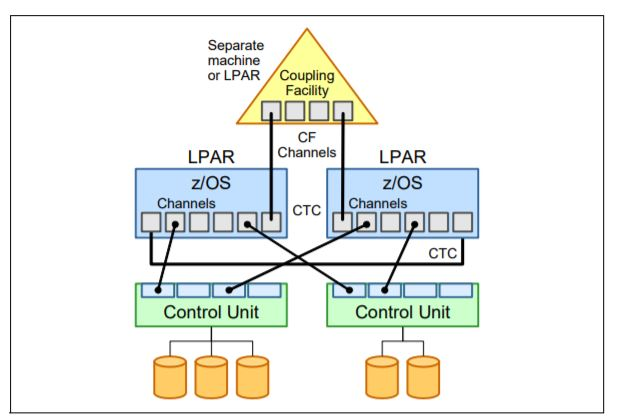
\includegraphics{img/ParallelSysplex}
	\caption[Visualisatie van een Parallel Sysplex]{{\small \textit{Visualisatie van een parallel sysplex met 2 LPARs en 1 Coupling Facility. Control Units controleren de logica voor bepaalde I/O-apparaten zoals printers of opslagfaciliteiten.(\cite{Ebbers2011})}}}
	\label{fig:parallelsysplex}
\end{figure}

Een goed geconfigureerde parallel sysplex cluster(zie figuur \ref{fig:parallelsysplex}) is zodanig ontworpen dat het een hoge beschikbaarheid biedt met een minimale onbeschikbaarheid. Dit is dus al een van technieken die de mainframe zijn hoge availabilty garanderen. Bijvoorbeeld: wanneer een systeem uitvalt, dan kan een ander systeem dit direct opvangen omdat alle data en kritische applicaties gedeeld worden in de parallel sysplex. De taken van het uitvallende systeem worden overgenomen. Ondertussen kan het gefaalde systeem herstart worden. Dit zorgt er uiteindelijk voor dat een laag aantal single points of failure aanwezig is binnen de sysplex. (\cite{Ebbers2011})

Een voorbeeld van een single point of failure(SPOF): Stel dat er een paar datasets van de coupling facility zijn die allebei op dezelfde fysieke drive staan, zouden die er bij een uitval van de CF LPAR niet meer toegankelijk zijn. In de parallel sysplex wordt dit vermeden door deze data te delen over meerder LPARs. Hiervoor bestaat bijvoorbeeld ook een check(XCF\_CDS\_SPOF)(\cite{IBMCorporation2019}).

\section{z/OS}
\label{subsec:z/OS}

Een ander belangrijk component van elke computer is het besturingssysteem. In het geval van deze proef is dat z/OS. Dit niet het enige maar wel het meest gebruikte besturingssysteem op de mainframe. Zoals de naam het zelf zegt draait ook z/OS Health Checker op dit besturingssysteem. Daarom bespreken we ook dit besturingssysteem. Een besturingssysteem is eigenlijk een collectie van programma's die de interne werking van het computer systeem beheren. Een besturingssysteem is ontworpen om er voor te zorgen dat de resources van de computer optimaal gebruikt worden.

z/OS is vandaag een resultaat van tientallen jaren technologische vooruitgang door IBM. Het begon als een besturingssysteem dat maar 1 programma tegelijk kon afhandelen naar een dat vandaag duizenden programma's en gebruikers tegelijk kan afhandelen. Het besturingssysteem wordt uitgevoerd in de processor en bevindt zich ook in de processor storage(zie figuur \ref{fig:omgevingzos}). Mainframe hardware bestaat uit een aantal processors en gekoppelde toestellen zoals DASD(Direct Acces storage devices de mainframe term voor hard disks). Die worden dan allemaal aangestuurd vanuit de consoles gekoppeld aan de mainframe. De DASD's worden gebruikt voor systeem functies of door programma's van gebruikers die uitgevoerd worden door z/OS. (\cite{Ebbers2011})


z/OS maakt het ook mogelijk om aan multiprocessing en multiprogramming te doen. Hierdoor is z/OS geschikt voor het uitvoeren van programma's die veel input/output operaties nodig hebben. 

\subsubsection{Multiprocessing}
\label{subsubsec:Multiprocessing}
Dit is het simultaan opereren van meerdere processors die meerdere hardware resources delen zoals memory of externe opslag

\subsubsection{Multiprogramming}
\label{subsubsec:Multiprogramming}
Multiprogramming laat z/OS toe om duizenden programma's te draaien voor gebruikers die werken aan verschillende projecten waar men zich ook bevindt op de wereld. Dit komt doordat z/OS het mogelijk maakt om belangrijke data van een onderbroken programma op te slagen, zodat men een ander programma kan uitvoeren. Als het onderbroken programma terug klaar is om uit te voeren kan het gewoon verder doen vanaf het punt van de onderbreking.(\cite{Ebbers2011})

\begin{figure}[h]
	\centering
	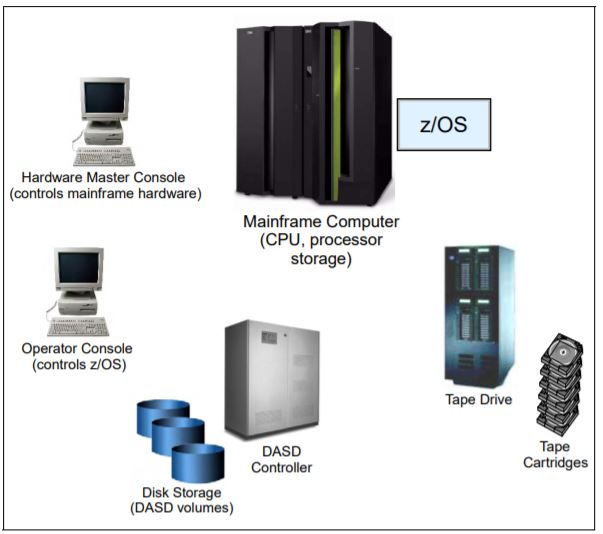
\includegraphics{img/Omgeving_zOS}
	\caption[z/OS binnen de mainframe omgeving]{{\small \textit{z/OS binnen de hardware omgeving bevindt zich op de mainframe. En wordt aangestuurd door aangesloten consoles/terminals. Om dan de data te bewerken op tape drives of DASD(term voor hard disk binnen de mainframe wereld). (\cite{Ebbers2011})}}}
	\label{fig:omgevingzos}
\end{figure}

\subsection{Storage gebruik van z/OS}
\label{subsec:Storage gebruik van z/OS}

z/OS heeft ook zijn eigen manier voor het gebruik van opslag/storage. Dit is ook belangrijk, omdat de term 'address space' gebruikt zal worden binnen deze proef. En die term is een techniek die z/OS gebruikt binnen de storage omgeving.

Een mainframe en een gewone computer hebben 2 soorten fysieke opslag:

\begin{itemize}
	\item Fysieke storage die zich bevindt op de mainframe processor zelf, ook wel 'real storage' genoemd te vergelijken met RAM op je laptop.
	\item Fysieke storage die zich buiten de mainframe bevindt op een tape of disk drive, dit wordt de auxiliary storage genoemd.
\end{itemize}

z/OS gebruikt deze 2 soorten storage om een andere soort te vormen namelijk virtual storage. Virtual storage is een combinatie van real en auxiliary storage. Het gebruikt een serie van tabellen en indexen om locaties binnen het real geheugen te associëren met locaties in de auxiliary storage.

Een address space is eigenlijk een range van virtuele adressen dat het besturingssysteem toekent aan een programma of gebruiker. Voor een gebruiker kan dit beschouwd worden als een container waar zijn data in zit. Door deze addres space moet z/OS niet een heel programma naar de real storage laden om het uit te voeren. Daarom zal men het programma in stukken(ook gekend als pages) van de auxiliary storage naar de real storage verplaatsen in de volgorde die nodig is om het prorgamma uit te voeren. Eens dat een page niet meer nodig is kan men het terugschrijven naar de auxiliary storage. Dit laat z/OS toe om meer programma's simultaan uit te voeren.

De fysieke opslag is daarom opgedeeld in verschillende stukken die elke hun eigen adres hebben maar de pages worden opgevraagd met hun virtueel adres. Het proces om een virtueel adres te vertalen in een real address noemt men Dynamic Address translation(DAT)(zie figuur \ref{fig:storage}). (\cite{Ebbers2011})

\begin{figure}[h]
	\centering
	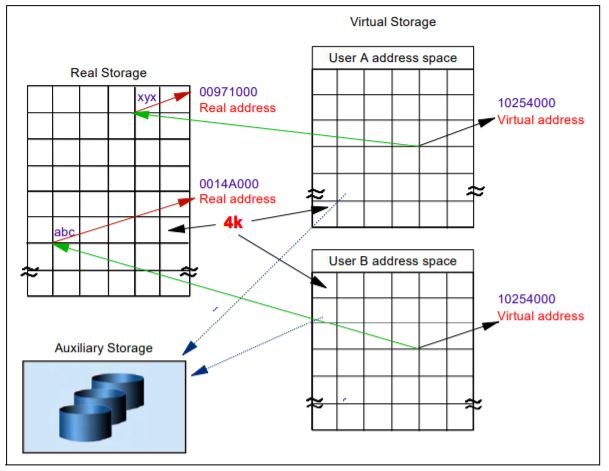
\includegraphics{img/Storage}
	\caption[Visualisatie van het concept van virtuele storage]{{\small \textit{Bijna alle programma's gebruiken virtuele adressen als ze refereren naar data in de real storage. Maar als een aangevraagd adres zich niet in de real storage bevindt zal er een onderbreking plaatsvinden en zal men de nodige data uit auxiliary storage naar de real storage laden(ook wel paging genoemd)(\cite{Ebbers2011})}}}
	\label{fig:storage}
\end{figure}

Een andere manier om te denken aan een address space is eigenlijk een soort van kaart voor de programmeur waarmee hij al zijn code en data kan opvragen.

\section{Interactie met z/OS}
\label{sec:interactie met z/OS}

Om een systeem te beheren moeten we er natuurlijk ook op kunnen aanloggen om zo bijvoorbeeld programma's te schrijven of bestanden te manipuleren. Voor deze interactie gebruikt men bijvoorbeeld een TSO/E commando om aan te loggen en dan ISPF, een collectie van menu's en panels die brede range van functies aanbied.

\subsection{Time Sharing Option/Extensions en Interactive System Productivity Facility}
\label{subsec:Time Sharing Option}

TSO/E of Time Sharing Option/Extensions laat gebruikers toe om een interactieve sessie te maken met een z/OS systeem. Hierdoor kunnen ze aanloggen op het z/OS systeem en gebruik maken van een command prompt interface. Maar omdat de command prompt niet echt handig is wordt er meestal gebruik gemaakt van de Interactive System Productivity Facility (ISPF). Dit is een collectie van menu's en panelen die een wijde range van functies aanbied voor het bewerken van data in z/OS. Zo biedt ISPF onder andere een tekst editor aan en functies voor het vinden en oplijsten van bestanden(zie figuur \ref{fig:ispf}). (\cite{Parziale2017})

\begin{figure}[h]
	\centering
	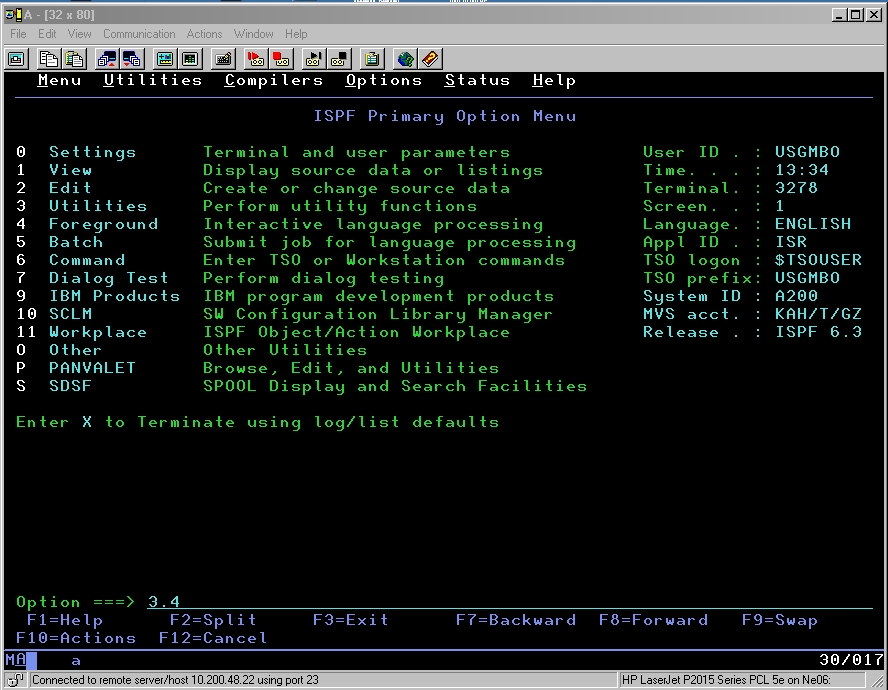
\includegraphics[width=0.7\linewidth]{img/IPSF}
	\caption[ISPF hoofdmenu]{{\small \textit{Dit is het hoofdmenu van ISPF vanaf hier kan je de verschillende panelen gebruiken}}}
	\label{fig:ispf}
\end{figure}

De bestanden binnen z/OS worden ook wel 'data sets' genoemd, dit is de term die ook verder gebruikt zal worden als we over bestanden spreken binnen z/OS. Er zijn 2 soorten data sets waarmee gewerkt word in deze proef.

\begin{itemize}
	\item Sequential data set: dit zijn data sets waarvan de individuele records georganiseerd zijn op hun fysieke volgorde binnen de dataset.
	\item Partitioned data set(PDS): dit is een data set die verdeeld is in partities ook wel 'members' deze kunnen een programma bevatten of gewoon data. Eigenlijks is een PDS een collectie van sequentiële data sets. Je zou het dus kunnen vergelijken met een folder met bestanden.
\end{itemize}

\section{Job Control Language en Job Entry Subsystem}
\label{sec:Job Control Language en Job Entry Subsystem}

In deze proef worden ook Jobs uitgevoerd voor het opstellen van de logs van z/OS Health Checker. Hiervoor wordt de Job Control Language(JCL) gebruikt. Want om een programma uit te voeren moet het verwerkt worden door z/OS.

Vooraleer het z/OS systeem een programma kan uitvoeren moet men een paar dingen doen. Eerst moet er beschreven worden welk programma men wil uitvoeren maar ook welke resources er gebruikt zullen worden(bv: eventuele input). Dit doet men aan de hand can een JCL ob. Deze jobs wordt gesubmit naar het Job Entry Subsystem(JES). Het JES zal deze jobs dan inplannen en uitvoeren en zal tot slot hun output verwerken(zie figuur \ref{fig:jes}). (\cite{Cosimo2018})

\begin{figure}[h]
	\centering
	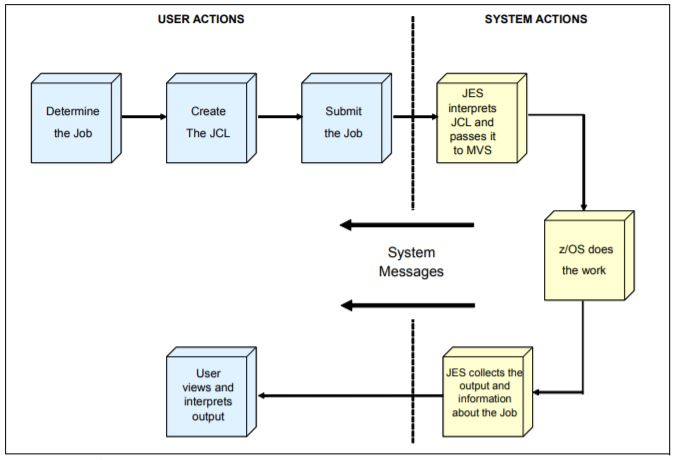
\includegraphics{img/JES}
	\caption[Visualisatie van JCL en JES]{{\small \textit{De gebruiker definieert, maakt en zal een job submitten. Deze wordt dan verwerkt door het Job Entry Subsystem en zal de output van de job teruggeven als resultaat.(\cite{Cosimo2018})}}}
	\label{fig:jes}
\end{figure}

\section{System Display and Search Facility}
\label{sec:System Display and Search Facility}

We willen natuurlijk de output van onze jobs kunnen zien daarvoor wordt er gebruikt gemaakt van de System Display and Search Facility of SDSF. Dit is niet het enige dat we kunnen zien in SDSF. Voor z/OS Health Checker zullen we ook deze tool gebruiken om alle info van het systeem op te vragen. Deze functie kan je bereiken via het hoofdmenu van ISPF met de optie 'S'(zie figuur \ref{fig:ispf} )

In SDSF zijn er veel panelen en soorten output die je kan opvragen maar de enige die wij zullen gebruiken is namelijk die van z/OS Health Checker die bereik je binnen SDSF via de 'ck' optie. Verder zal je bij het schrijven van jobs het 'Status of jobs' paneel nodig hebben. Dit panel toont de output van uitgevoerde jobs, dit paneel bereik je met de 'st' optie(zie figuur \ref{fig:sdsf}).

\begin{figure}[h]
	\centering
	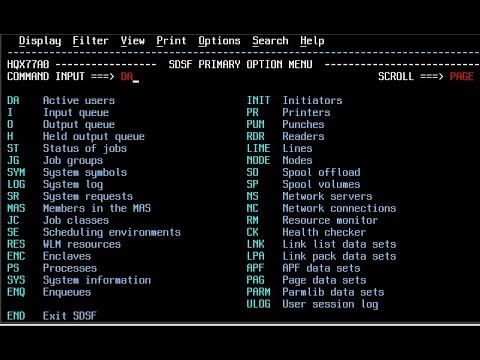
\includegraphics[width=0.7\linewidth]{img/SDSF}
	\caption[SDSF Hoofdmenu]{{\small \textit{Hier zie je het hoofdmenu van SDSF en onder andere ook de 2 opties die gebruikt worden doorheen de proef namelijk 'ck' en 'st'}}}
	\label{fig:sdsf}
\end{figure}

 
\section{De Parmlib}
\label{sec:De Parmlib}

z/OS Health Checker heeft ook enkele datasets in de parmlib die veranderd worden in deze proef daarom moeten we ook begrijpen wat die parmlib eigenlijk is. Elk z/OS systeem heeft een PDS met members die worden meegegeven door IBM. Deze PDS is SYS1.PARMLIB. De members zijn allemaal systeem en applicatie parameters die het systeem nodig heeft bij het opstarten(Initial Program Load(IPL) in mainframe term). Bij de IPL wordt de parmlib gelezen om het systeem op te zetten. Deze PDS wordt later ook nog gelezen door andere componenten en programma's. (\cite{Cosimo2018})
 
Een van deze componenten is z/OS Health Checker. In de parmlib zitten members die definiëren welke controles (Checks) er zullen uitgevoerd worden en welke niet.
 
\section{z/OS Health Checker}
\label{sec:z/OS Health Checker}

Na een analyse naar de oorzaken van de verschillende uitvallen kwam men tot de conclusie dat veel hiervan perfect vermeden had kunnen worden. Vele uitvallen kwamen door slechte configuraties die leiden tot single points of failure. Hierdoor is z/OS Health Checker ontwikkelt door IBM. (\cite{Walle2013})

IBM Health Checker voor z/OS is een tool die helpt om potentiële problemen op te sporen in de configuratie van het systeem. Deze problemen zouden een grote impact kunnen hebben op het systeem of zouden zelfs een uitval kunnen veroorzaken. Health Checker kijkt de huidige instellingen van z/OS en de Sysplex na en vergelijkt deze met instellingen die door IBM aangeraden worden. Bij eventuele problemen zal Health Checker een output genereren met gedetailleerde info over het probleem zelf en op welke manier je het probleem het beste oplost. Wel belangrijk is dat Health Checker eerder een preventieve tool is en geen monitoring tool. (\cite{Bezzi2010})

z/OS Health Checker bestaat uit 2 delen
\begin{itemize}
	\item De checks
	\item Het framework	
\end{itemize}

\subsection{Health Checker Framework}
\label{subsec:Health Checker Framework}

Het framework van z/OS Health Checker is de interface die je gebruikt om checks uit te voeren en te beheren. Deze ondersteunt niet enkele checks van IBM maar ook die van software producenten zoals Computer Associates en Compuware. Binnen het framework zit de HZSPQE data, hierin zit alle informatie die een check nodig zou hebben zoals de default parameters.  Het framework bevat ook de Message table die de data bijhoudt van de output van de checks(zie figuur \ref{fig:hcframework}). (\cite{IBMCorporation2019})

\begin{figure}[h]
	\centering
	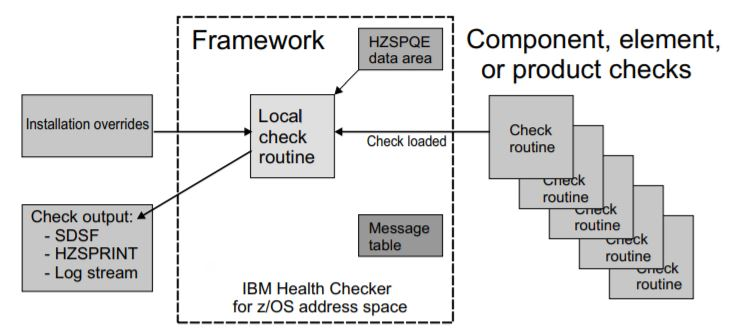
\includegraphics[width=0.7\linewidth]{img/HCFramework}
	\caption[z/OS Health Checker Framework]{{\small \textit{Het z/OS Health Checker Framework dat het mogelijk maakt om checks uit te voeren en de output hiervan door te geven aan SDSF en andere tools.(\cite{IBMCorporation2019})}}}
	\label{fig:hcframework}
\end{figure}


\subsection{De Checks}
\label{sec:z/OS Health Checker Checks}

De Checks zelf zijn programma's die componenten en instellingen evalueren en dan eventuele problemen melden. Deze checks worden voornamelijk aangeboden door IBM zelf maar deze kunnen ook van andere bedrijven zijn. Je kan ook zelf Checks schrijven met System REXX. Een check vergelijkt de instellingen van 1 bepaald component met een set van instellingen die aangeraden worden door de eigenaar van de check. De aangeraden instellingen zijn geen verplichte instellingen maar eerder een best practice van IBM. Je kan deze ook zelf definiëren of aanpassen. (\cite{Bezzi2010})

Een check wordt gedefinieerd met 3 waarden

\subsubsection{Check Owner}
\label{subsubsec:Check Owner}

Elke check heeft zijn eigenaar. De naam van de check is meestal verbonden met het component waarvoor hij draait. In deze naam zit ook bijna altijd een verwijzing naar het bedrijf of product die de check gemaakt heeft. De checks van IBM beginnen dan ook allemaal met IBM. Een check owner is een string van maximum 16 karakters. Een voorbeeld van een check owner is bijvoorbeeld IBMXCF. Deze check is dus geschreven door IBM en zal iets te maken hebben met XCF(Cross-system Coupling Facility). Een check owner heeft meerdere checks zelf. (\cite{Bezzi2010})

\subsubsection{Check Name}
\label{subsubsec:Check Name}

De check zelf heeft natuurlijk ook een naam. En is uniek voor elke check. Deze zal maximum 32 karakters lang zijn. Een voorbeeld van een check naam: "XCF\_CDS\_MAXSYSTEM".

\subsubsection{Check Values}
\label{subsubsec:Check Values}

Een check bezit verder ook nog enkele vooraf gedefinieerde waarden

\begin{enumerate}
	\item Een interval die definieert hoe vaak en wanneer de check uitgevoerd wordt.
	\item De ernst(Severity) van een check die de check output definieert. Hoe grotere het potentiële probleem hoe hoger de severity. 
\end{enumerate}

\subsubsection{Check Types}
\label{subsubsec:Check Type}

Verder zijn er ook 3 types van checks: Local, remote en REXX checks. In deze proef komen enkel de local checks aan bod. De lokale check is geschreven in ASSEMBLER voor z/OS. En draaien binnen de Health Checker address space.Deze worden opgeroepen met parameters die verwijzen naar de HZSPQE data. In de HZSPQE data zit alle data die de check routine nodig heeft. Het verschil met een Remote check is dat een remote check niet binnen de address space van Health Checker draait. 

\subsubsection{Check Output}
\label{subsubsec:Check Output}

 De check output is ook zeer belangrijk. Deze duidt namelijk aan of een check al dan niet succesvol was. Er zijn verschillende soorten check messages.

\begin{itemize}
	\item Information Message: Deze message krijg je wanneer een check succesvol is of wanneer deze niet kan draaien in de huidige omgeving(Bijvoorbeeld wanneer het component dat de check evalueert niet aanwezig is op het systeem).
	\item Exception Message: Deze message krijg je wanneer de check onsuccesvol was en deze een potentieel probleem heeft gevonden. Dit noemt men een exception. Dit bericht bevat de severity van het probleem samen met suggesties om het probleem op te lossen
	\item Report: Bij een exception zal er ook een extra report bijgevoegd worden met extra informatie over het probleem.
	\item Debug: Sommige checks kan je in debug mode uitvoeren. Dit wordt vooral gebruikt bij het ontwikkelen van een eigen check.
\end{itemize}

Voor een voorbeeld van check output zie bijlage \ref{sec:Check Output}

\subsubsection{Check Status}
\label{subsubsec:Check Status}

Een check heeft ook een bepaalde status. Deze status duid aan of een check al dan niet geactiveerd is. Volgende statussen zijn mogelijk. (\cite{IBM2019})

\begin{itemize}
	\item ACTIVE: Dit specifieert dat de check actief is en draait.
	\item INACTIVE: Dit specifieert dat de check niet actief is en deze niet zal draaien.
	\item Ook al is een check actief of inactief kan deze ook nog 2 opties hebben namelijk Enabled \& Disabled. Wanneer een check enabled is betekent dat dat deze kan draaien binnen de huidige omgeving. Als een check disabled is kan dit betekenen dat deze niet kan draaien omdat er condities binnen de huidige parallel sysplex omgeving zijn die dat verhinderen. Bijvoorbeeld een check van DB2 die disabled staat omdat er op een bepaalde LPAR geen DB2 product is.
	\item GLOBAL: Dit betekent dat de check globaal is en daarom maar op 1 LPAR mag draaien van de gehele sysplex. Maar de check zal wel instellingen controleren voor de hele parallel sysplex. 
\end{itemize}


Verder is er nog 1 speciaal soort check. Namelijk de migration check. Deze check kan je helpen bij het plannen voor een overschakelen van z/OS versie. Deze checks kan je uitvoeren na een migratie om te kijken of deze succesvol was. Of voor een migratie om te kijken of je systeem klaar is voor een upgrade. Deze checks beginnen altijd met 'ZOSMIG'. (\cite{IBMCorporation2019})

%%=============================================================================
%% Methodologie
%%=============================================================================

\chapter{\IfLanguageName{dutch}{Methodologie}{Methodology}}
\label{ch:methodologie}

%% TODO: Hoe ben je te werk gegaan? Verdeel je onderzoek in grote fasen, en
%% licht in elke fase toe welke stappen je gevolgd hebt. Verantwoord waarom je
%% op deze manier te werk gegaan bent. Je moet kunnen aantonen dat je de best
%% mogelijke manier toegepast hebt om een antwoord te vinden op de
%% onderzoeksvraag.

\lipsum[21-25]



% Voeg hier je eigen hoofdstukken toe die de ``corpus'' van je bachelorproef
% vormen. De structuur en titels hangen af van je eigen onderzoek. Je kan bv.
% elke fase in je onderzoek in een apart hoofdstuk bespreken.

%\input{...}
%\input{...}
%...

%%=============================================================================
%% Conclusie
%%=============================================================================

\chapter{Conclusie}
\label{ch:conclusie}

% TODO: Trek een duidelijke conclusie, in de vorm van een antwoord op de
% onderzoeksvra(a)g(en). Wat was jouw bijdrage aan het onderzoeksdomein en
% hoe biedt dit meerwaarde aan het vakgebied/doelgroep? 
% Reflecteer kritisch over het resultaat. In Engelse teksten wordt deze sectie
% ``Discussion'' genoemd. Had je deze uitkomst verwacht? Zijn er zaken die nog
% niet duidelijk zijn?
% Heeft het onderzoek geleid tot nieuwe vragen die uitnodigen tot verder 
%onderzoek?

\lipsum[76-80]



%%=============================================================================
%% Bijlagen
%%=============================================================================

\appendix
\renewcommand{\chaptername}{Appendix}

%%---------- Onderzoeksvoorstel -----------------------------------------------

\chapter{Onderzoeksvoorstel}

Het onderwerp van deze bachelorproef is gebaseerd op een onderzoeksvoorstel dat vooraf werd beoordeeld door de promotor. Dat voorstel is opgenomen in deze bijlage.

% Verwijzing naar het bestand met de inhoud van het onderzoeksvoorstel
\input{../voorstel/voorstel-inhoud}

\renewcommand{\chaptername}{Bijlangen}
\chapter{Bijlagen}

%%---------- Andere bijlagen --------------------------------------------------
% TODO: Voeg hier eventuele andere bijlagen toe
\section{Check Output}
\label{sec:Check Output}

Check output bij exception van de XCF\_CF\_STR\_POLICIYSIZE check.

\verbatiminput{checkOutput/output.txt}

\section{Tabellen Standaard opstelling z/OS Health Checker}
\label{sec:Tabellen Standaard opstelling z/OS Health Checker}

Dit zijn de tabellen van alle checks gegroepeerd per team dat beheer heeft over de checks.


In deze bijlage bevinden zich de tabellen met de standaardopstelling van de checks van volgende teams in deze volgorde

\begin{enumerate}
	\item CICS
	\item Communication
	\item Print
	\item Automation
	\item Rollout \& Operate
	\item Runtime Control
	\item Security
	\item SOE
	\item Storage
	\item zOPEN
	\item DB
\end{enumerate}

De tabellen staan horizontaal omdat ze verticaal niet op een pagina passen.

\begin{landscape}
	\begin{table}[h]
		\begin{tabular}{|l|l|l|p{5cm}|l|l|}
			\hline
			\textbf{Name}                    & \textbf{Status}            & \textbf{Outcome} &\textbf{ Reason} & \textbf{Run} & \textbf{00/\&SUF.} \\ \hline
			CICS\_CEDA\_ACCES       & INACTIVE(ENABLED) & INACT   & CEDA   can be used by unauthenticated users                                        & No  & 00        \\ \hline
			CICS\_JOBSUB\_SPOOL     & INACTIVE(ENABLED) & INACT   & Jobs   can be run with regionid authority by unauthenticated users using the SPOOL & No  & 00        \\ \hline
			CICS\_JOBSUB\_TDQINTRDR & INACTIVE(ENABLED) & INACT   & Jobs   can be run with regionid authority by unauthenticated users using a TDQ     & No  & 00        \\ \hline
		\end{tabular}
	\end{table}
\end{landscape}

\begin{landscape}
	\begin{table}[h]
		\begin{tabular}{|l|l|l|p{4.5cm}|l|l|}
			\hline
			\textbf{Name}                       & \textbf{Status}   & \textbf{Outcome} & \textbf{Reason}                                                                                                & \textbf{Run} & \textbf{00/\&SUF.} \\ \hline
			CSAPP\_FTPD\_ANONYMOUS\_JES         & ACTIVE(ENABLED)   & SUCCES           & CHECK   FTPD ANONYMOUS JES STATEMENT IS IN USE                                                                 & Yes          & N/A                \\ \hline
			CSAPP\_FTPDMVRSHD\_RHOSTS\_DATA     & ACTIVE(ENABLED)   & SUCCES           & CHECK   MVRSHD RHOSTS DATA IS IN USE                                                                           & Yes          & N/A                \\ \hline
			CSAPP\_SNMPAGENT\_PUBLIC\_COMMUNITY & ACTIVE(ENABLED)   & SUCCES           & CHECK   SNMP AGENT PUBLIC COMMUNITY IS IN USE                                                                  & Yes          & N/A                \\ \hline
			CSRES\_AUTOQ\_GLOBALTCPIPDATE       & ACTIVE(ENABLED)   & SUCCES           & CHECK   THAT GLOBALTCPIPDATA IS NOT    SPECIFIED   WHEN AUTOQUIESCE IS SPECIFIED                               & Yes          & N/A                \\ \hline
			CSRES\_AUTOQ\_RESOLVEVIA            & ACTIVE(ENABLED)   & SUCCES           & CHECK   RESOLVEVIA VALUE WHEN THE AUTONOMIC QUIESCING OF UNRESPONSIVE NAME SERVERS FUNCTION IS ACTIVE          & Yes          & N/A                \\ \hline
			CSRES\_AUTOQ\_TIMEOUT               & ACTIVE(ENABLED)   & SUCCES           & CHECK   RESOLVEVIA VALUE WHEN THE AUTONOUTONOMIC QUIESCING OF UNRESPONSIVE   NAME   SERVERS FUNCTION IS ACTIVE & Yes          & N/A                \\ \hline
			CSTCP\_CINENT\_PORTRNG\_RSV\_TCPIP* & INACTIVE(ENABLED) & INACT            & CHECK   THAT CINET INADDRANYPORT RANGE IS   RESERVED   FOR OMVS ON THE TCP/IP STACK                            & No           & 00                 \\ \hline
		\end{tabular}
	\end{table}
\end{landscape}

\begin{landscape}
	\begin{table}[h]
		\begin{tabular}{|l|l|l|p{4.5cm}|l|l|}
			\hline
			CSTCP-IPMAXRT4\_TCPIP*           & ACTIVE(ENABLED)  & SUCCES & CHECK   FOR TCP/IP IPV4 INDIRECT ROUTES    MAXIMUM   THRESHOLD                      & Yes & N/A \\ \hline
			CSTCP-IPMAXRT6\_TCPIP*           & ACTIVE(ENABLED)  & SUCCES & CHECK   FOR TCP/IP IPV6 INDIRECT ROUTES    MAXIMUM   THRESHOLD                      & Yes & N/A \\ \hline
			CSTCP\_IWQ\_IPSEC\_TCPIP*        & ACTIVE(ENABLED)  & SUCCES & ENSURE SUFFICIENT FIXED STORAGE IS   AVAILABLE FOR IWQ IPSEC                        & Yes & N/A \\ \hline
			CSTCP\_SYSPLEXMON\_RECOV\_TCPIP* & ACTIVE(ENABLED)  & SUCCES & CHECK   THAT SYSPLEXMONITOR RECOVERY IS    SPECIFIED   WHEN DYNAMICXCF IS SPECIFIED & Yes & N/A \\ \hline
			CSTCP\_SYSTCPIP\_CTRACE\_TCPIP*  & ACTIVE(ENABLED)  & SUCCES & CHECK   FOR TCP/IP SYSTCPIP CTRACE WITH   NONDEFAULT   OPTION                       & Yes & N/A \\ \hline
			CSTCP\_TCPMAXRCVBUFRSIZE\_TCPIP* & ACTIVE(ENABLED)  & SUCCES & ENSURE   TCP RECEIVE BUFFER SIZE IS    SUFFICIENT   FOR FTP SERVER                  & Yes & N/A \\ \hline
			CSVTAM\_CSM\_STG\_LIMIT          & ACTIVE(ENABLED)  & SUCCES & CHECK CSM STORAGE LIMIT    VTV0022 REXX?                                            & Yes & N/A \\ \hline
			CSVTAM\_T1BUF\_T2BUF\_EE         & ACTIVE(ENABLED)  & SUCCES & CHECK   T1BUF/T2BUF ALLOCATIONS WITH EE                                             & Yes & N/A \\ \hline

		\end{tabular}
	\end{table}
\end{landscape}

\begin{landscape}
	\begin{table}[h]
		\begin{tabular}{|l|l|l|p{4.5cm}|l|l|}
			\hline
			CSVTAM\_T1BUF\_T2BUF\_NOEE    & ACTIVE(DISABLED) & ENV N  & CHECK T1BUF/T2BUF ALLOCATIONS WITHOUT EE &Yes & N/A \\ \hline
			CSVTAM\_VIT\_OPT\_ALL         & ACTIVE(ENABLED) & SUCCES & CHECK   VIT OPT=ALL IS NOT SPECIFIED     & Yes & N/A \\ \hline
			CSVTAM\_VIT\_OPT\_STDOPTS     & ACTIVE(ENABLED) & SUCCES & CHECK   VIT STDOPTS OPTION IS ACTIVE     & Yes & N/A \\ \hline
			TPX\_ACB\_INACTIVE\_@TPX*     & ACTIVE(ENABLED) & SUCCES & TPX ACB   is inactive                    & Yes & N/A \\ \hline
			TPX\_CF\_UNCONNECTED\_@TPX*   & ACTIVE(ENABLED) & SUCCES & TPX   coupling facility is not connected & Yes & N/A \\ \hline
			TPX\_STORAGE\_OVERFLOW\_@TPX* & ACTIVE(ENABLED) & SUCCES & TPX   storage overflow beyond boundries  & Yes & N/A \\ \hline
		\end{tabular}
	\end{table}
\end{landscape}

\begin{landscape}
	\begin{table}[h]
		\begin{tabular}{|l|l|l|p{4.5cm}|l|l|}
			\hline
			\textbf{Name}               & \textbf{Status} & \textbf{Outcome} & \textbf{Reason}                                                                            & \textbf{Run} & \textbf{00/\&SUF.} \\ \hline
			DLVR\_CKPT\_USAGE@RMOVT1    & ACTIVE(ENABLED) & SUCCES           & Monitor   CA Deliver checkpoint utilization.                                               & Yes          & N/A                \\ \hline
			DLVR\_OPT\_HDETAIL@RMOVT1   & ACTIVE(ENABLED) & SUCCES           & Insure   the HDETAIL option is only activated when necessary                               & Yes          & N/A                \\ \hline
			DLVR\_PRFM\_PQE@RMOVT1      & ACTIVE(ENABLED) & SUCCES           & Monitor   CA Deliver application work queues.                                              & Yes          & N/A                \\ \hline
			SPOOL\_CKPT\_ACT@ESF        & ACTIVE(ENABLED) & SUCCES           & To   check CA Spool checkpoint working                                                     & Yes          & N/A                \\ \hline
			SPOOL\_FILE\_QUEUE\_PCT@ESF & ACTIVE(ENABLED) & SUCCES           & To   check CA Spool file queue utilization                                                 & Yes          & N/A                \\ \hline
			SPOOL\_SPACE\_PCT@ESF       & ACTIVE(ENABLED) & SUCCES           & To   check CA Spool data set space utilization                                             & Yes          & N/A                \\ \hline
			SPOOL\_TCP\_ACT@ESF         & ACTIVE(ENABLED) & SUCCES           & To   check CA Spool TCP/IP printer subtasks                                                & Yes          & N/A                \\ \hline
			SPOOL\_TRANSFRM\_ACT@ESF    & ACTIVE(ENABLED) & SUCCES           & To   check CA Spool Transformer subtasks                                                   & Yes          & N/A                \\ \hline
			VIEW\_OPT\_CLFMDST@SAR*     & ACTIVE(ENABLED) & SUCCES           & Alert   datacenter staff that CA View is configured to archive every report in the   spool & Yes          & N/A                \\ \hline
			VIEW\_OPT\_MASTER@SAR*      & ACTIVE(ENABLED) & SUCCES           & Insure   that all CA View users do not have access to ADMINISTRATIVE functions             & Yes          & N/A                \\ \hline
			VIEW\_OPT\_TBACKUP@SAR*     & ACTIVE(ENABLED) & SUCCES           & Insure   that TBACKUP is set to a value that allows the database to be restored            & Yes          & N/A                \\ \hline
		\end{tabular}
	\end{table}
\end{landscape}

\begin{landscape}
	\begin{table}[h]
		\begin{tabular}{|l|l|l|p{4.5cm}|l|l|}
			\hline
			\textbf{Name}             & \textbf{Status}  & \textbf{Outcome} & \textbf{Reason}                                 & \textbf{Run} & \textbf{00/\&SUF.} \\ \hline
			GDPS\_CHECK\_CONFIG       & ACTIVE(ENABLED)  & EXCEPTION        & GDPS check verifies configurations              & Yes          & N/A                \\ \hline
			GDPS\_CHECK\_CONSOLE      & ACTIVE(ENABLED)  & SUCCES           & GDPS   check CONSOLE information                & Yes          & N/A                \\ \hline
			GDPS\_CHECK\_DASDMIH      & ACTIVE(ENABLED)  & SUCCES           & GDPS   check DASD MIH                           & Yes          & N/A                \\ \hline
			GDPS\_CHECK\_DEVICE       & ACTIVE(ENABLED)  & EXCEPTION        & GDPS   check verifies device configuration      & Yes          & N/A                \\ \hline
			GDPS\_CHECK\_GRS          & ACTIVE(DISABLED) & ENV N            & GDPS check verifies GRS definitions             & Yes          & N/A                \\ \hline
			GDPS\_CHECK\_JOBS         & ACTIVE(ENABLED)  & SUCCES           & GDPS   check JOBS                               & Yes          & N/A                \\ \hline
			GDPS\_CHECK\_K\_SYS\_LPAR & ACTIVE(DISABLED) & ENV N            & GDPS check K SYS LPAR informationx              & Yes          & N/A                \\ \hline
			GDPS\_CHECK\_LOGR         & ACTIVE(ENABLED)  & SUCCES           & GDPS   check verifies LOGR configuration        & Yes          & N/A                \\ \hline
			GDPS\_CHECK\_MAXSYS       & ACTIVE(ENABLED)  & SUCCES           & GDPS   check MAXSYS information                 & Yes          & N/A                \\ \hline
			GDPS\_CHECK\_NUMUCBS      & ACTIVE(ENABLED)  & SUCCES           & GDPS   max devices generated                    & Yes          & N/A                \\ \hline
		\end{tabular}
	\end{table}
\end{landscape}

\begin{landscape}
	\begin{table}[h]
		\begin{tabular}{|l|l|l|p{4.5cm}|l|l|}
			\hline
			GDPS\_CHECK\_SPOF         & ACTIVE(ENABLED)  & EXCEPTION        & GDPS check connectivity Single Point Of Failure & No           & 00                 \\ \hline
			GDPS\_CHECK\_STATE        & ACTIVE(ENABLED)  & SUCCES           & GDPS   check STATE                              & Yes          & N/A                \\ \hline
			GDPS\_CHECK\_XCF          & ACTIVE(ENABLED)  & SUCCES           & GDPS   check verifies XCF definitions           & Yes          & N/A                \\ \hline
			GDPS\_CHECK\_XCF\_CDS     & ACTIVE(ENABLED)  & SUCCES           & GDPS   check verify XCF CDS datasets            & Yes          & N/A                \\ \hline
		\end{tabular}
	\end{table}
\end{landscape}


\begin{landscape}
	\begin{table}[h]
		\begin{tabular}{|l|l|l|p{4.5cm}|l|l|}
			
		\end{tabular}
	\end{table}
\end{landscape}

\section{Parmlib members voor z/OS Health Checker}
\label{sec:Parmlin members voor z/OS Health Checker}

In deze bijlagen bevind zich de Parmlib members die aangemaakt zijn voor de standaardopstelling. HZSPRMT4 is de member die voortaan gebruikt zal worden bij het uitbreiden van de parallel sysplex.

\subsection{HZSPRM00}
\label{subsec:HZSPRM00}

\verbatiminput{Parmlib/HZSPRM00.txt}

\subsection{HZSPRMT1}
\label{subsec:HZSPRMT1}

\verbatiminput{Parmlib/HZSPRMT1.txt}

\subsection{HZSPRMT2}
\label{subsec:HZSPRMT2}

\verbatiminput{Parmlib/HZSPRMT2.txt}

\subsection{HZSPRMT3}
\label{subsec:HZSPRMT3}

\verbatiminput{Parmlib/HZSPRMT3.txt}

\subsection{HZSPRMT4}
\label{subsec:HZSPRMT4}

\verbatiminput{Parmlib/HZSPRMT4.txt}

\section{JCL jobs}
\label{sec:JCL jobs}

Dit zijn de JCL jobs die gebruikt worden voor het opstellen van de log die daarna doorgestuurd word via mail.

\subsection{FHZSVT11}
\label{subsec:FHZSVT11}

\verbatiminput{JCL/FHZSVT11.txt}

\subsection{FHZSVT21}
\label{subsec:FHZSVT21}

\verbatiminput{JCL/FHZSVT21.txt}

\subsection{FHZSVT31}
\label{subsec:FHZSVT31}

\verbatiminput{JCL/FHZSVT31.txt}

\subsection{FHZSVT41}
\label{subsec:FHZSVT41}

\verbatiminput{JCL/FHZSVT41.txt}

%%---------- Referentielijst --------------------------------------------------

\printbibliography[heading=bibintoc]

\end{document}
